
\subsection*{Cônicas Transladadas}
\begin{frame}[label=conicas]{Cônicas Transladadas}

\begin{center}
{\color{blue} Mudança de coordenadas }
\end{center}
\begin{equation*}
	\begin{cases}
		\textcolor{blue}{x'}=x-x_0\\
		\textcolor{blue}{y'}=y-y_0.
	\end{cases}
\end{equation*}

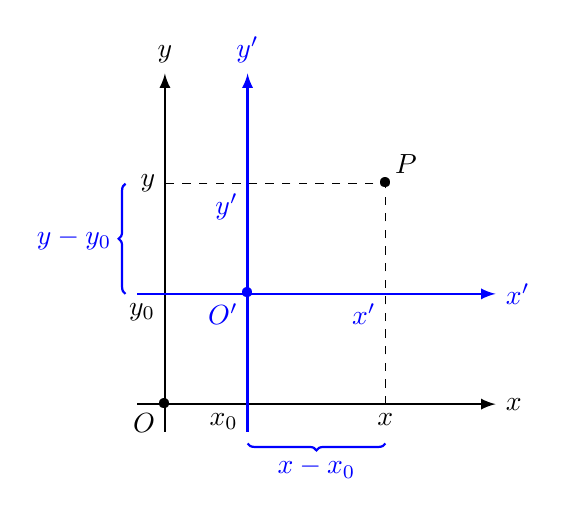
\begin{tikzpicture}[scale=0.7]

\usetikzlibrary{decorations.pathreplacing} 
\tikzset{>=latex}
%\draw[help lines, color=gray!30, dashed] (0,0) grid (6,6);

%sistema de eixos e ponto P
\draw[->,thick] (-.5,0)--(6,0) node[right]{$x$};
\draw[->,thick] (0,-.5)--(0,6) node[above]{$y$};
\node at (0,0) {\textbullet};
\node[below left] at (0,0) {$O$};
\node at (4,4) {\textbullet};
\node[above right] at (4,4) {$P$};
\draw[dashed] (4,0) -- (4,4) -- (0,4);
\node[below ] at (4,0) {$x$};
\node[left] at (0,4) {$y$};

%ponto de translação
\uncover<2->{
\node[blue] at (1.5,2) {\textbullet};
\node[below left,blue] at (1.5,2) {$O'$};
\node[below left] at (1.5,0) {$x_0$};
\node[below left] at (0,2) {$y_0$};
\draw[dashed] (1.5,0)--(1.5,2)--(0,2);
}


\uncover<3->{
\draw[->,thick,blue] (-.5,2)--(6,2) node[right]{$x'$};
\draw[->,thick,blue] (1.5,-.5)--(1.5,6) node[above]{$y'$};
}

\uncover<4->{
\node[below left,blue] at (4,2) {$x'$};
\node[below left,blue] at (1.5,4) {$y'$};

\draw[thick,decoration={brace,mirror,raise=0.5cm},decorate,blue] (1.5,0) --   (4,0)
node[pos=0.5,anchor=north,yshift=-0.55cm,blue] {$x-x_0$};
\draw[thick,decoration={brace,raise=0.5cm},decorate,blue] (0,2) --   (0,4)
node[pos=0.5,anchor=east,xshift=-0.55cm,blue] {$y-y_0$};}

\end{tikzpicture}


\end{frame}


\begin{frame}[label=conicas]

As equações de cônicas que não apresentam termos mistos da forma $xy$ 
podem  ser colocadas na forma reduzida através de uma translação de 
eixos.

\begin{exe}
Identifique e faça o esboço das cônicas a seguir:

\begin{enumerate}
\item $x^2+2y^2-6x+8y+9=0$.
\item $4x^2-16y^2-24x-24y+33=0$.
\end{enumerate}
\end{exe}

\end{frame}


